%
% Main document
% ===========================================================================
% This is part of the document "Project documentation template".
% Authors: brd3, kaa1
%

%---------------------------------------------------------------------------
\documentclass[
	a4paper,					% paper format
	10pt,							% fontsize
%	twoside,					% double-sided
	openright,				% begin new chapter on right side
	notitlepage,			% use no standard title page
	parskip=half,			% set paragraph skip to half of a line
]{scrreprt}					% KOMA-script report
%---------------------------------------------------------------------------

\raggedbottom
\KOMAoptions{cleardoublepage=plain}			% Add header and footer on blank pages


% Load Standard Packages:
%---------------------------------------------------------------------------
\usepackage[standard-baselineskips]{cmbright}

\usepackage[ngerman]{babel}										% german hyphenation
\usepackage[utf8]{inputenc}  							% Unix/Linux - load extended character set (ISO 8859-1)
%\usepackage[ansinew]{inputenc}  							% Windows - load extended character set (ISO 8859-1)
\usepackage[T1]{fontenc}											% hyphenation of words with ä,ö and ü
\usepackage{textcomp}													% additional symbols
\usepackage{ae}																% better resolution of Type1-Fonts 
\usepackage{fancyhdr}													% simple manipulation of header and footer 
\usepackage{etoolbox}													% color manipulation of header and footer
\usepackage{graphicx}                      		% integration of images
\usepackage{float}														% floating objects
\usepackage{caption}													% for captions of figures and tables
\usepackage{booktabs}													% package for nicer tables
\usepackage{tocvsec2}													% provides means of controlling the sectional numbering
\usepackage{tabularx}

%---------------------------------------------------------------------------

% Custom packages added by Roger
%---------------------------------------------------------------------------
\usepackage{listings}
\usepackage{pdflscape}

%---------------------------------------------------------------------------

% Load Math Packages
%---------------------------------------------------------------------------
\usepackage{amsmath}                    	   	% various features to facilitate writing math formulas
\usepackage{amsthm}                       	 	% enhanced version of latex's newtheorem
\usepackage{amsfonts}                      		% set of miscellaneous TeX fonts that augment the standard CM
\usepackage{amssymb}													% mathematical special characters
\usepackage{exscale}													% mathematical size corresponds to textsize
%---------------------------------------------------------------------------

% Package to facilitate placement of boxes at absolute positions
%---------------------------------------------------------------------------
\usepackage[absolute]{textpos}
\setlength{\TPHorizModule}{1mm}
\setlength{\TPVertModule}{1mm}
%---------------------------------------------------------------------------					
			
% Definition of Colors
%---------------------------------------------------------------------------
\RequirePackage{color}                          % Color (not xcolor!)
\definecolor{linkblue}{rgb}{0,0,0.8}            % Standard
\definecolor{darkblue}{rgb}{0,0.08,0.45}        % Dark blue
\definecolor{bfhgrey}{rgb}{0.41,0.49,0.57}      % BFH grey
%\definecolor{linkcolor}{rgb}{0,0,0.8}     			% Blue for the web- and cd-version!
\definecolor{linkcolor}{rgb}{0,0,0}        			% Black for the print-version!
%---------------------------------------------------------------------------

% Hyperref Package (Create links in a pdf)
%---------------------------------------------------------------------------
\usepackage[
	pdftex,ngerman,bookmarks,plainpages=false,pdfpagelabels,
	backref = {false},										% No index backreference
	colorlinks = {true},                  % Color links in a PDF
	hypertexnames = {true},               % no failures "same page(i)"
	bookmarksopen = {true},               % opens the bar on the left side
	bookmarksopenlevel = {0},             % depth of opened bookmarks
	pdftitle = {Template für Bachelor Thesis},	   	% PDF-property
	pdfauthor = {brd3},        					  % PDF-property
	pdfsubject = {LaTeX Template},        % PDF-property
	linkcolor = {linkcolor},              % Color of Links
	citecolor = {linkcolor},              % Color of Cite-Links
	urlcolor = {linkcolor},               % Color of URLs
]{hyperref}
%---------------------------------------------------------------------------
% Set up page dimension
%---------------------------------------------------------------------------
\usepackage{geometry}
\geometry{
	a4paper,
	left=28mm,
	right=15mm,
	top=30mm,
	headheight=20mm,
	headsep=10mm,
	textheight=242mm,
	footskip=15mm
}
%---------------------------------------------------------------------------

% Makeindex Package
%---------------------------------------------------------------------------
\usepackage{makeidx}                         		% To produce index
\makeindex                                    	% Index-Initialisation
%---------------------------------------------------------------------------

% Glossary Package
%---------------------------------------------------------------------------
% the glossaries package uses makeindex
% if you use TeXnicCenter do the following steps:
%  - Goto "Ausgabeprofile definieren" (ctrl + F7)
%  - Select the profile "LaTeX => PDF"
%  - Add in register "Nachbearbeitung" a new "Postprozessoren" point named Glossar
%  - Select makeindex.exe in the field "Anwendung" ( ..\MiKTeX x.x\miktex\bin\makeindex.exe )
%  - Add this [ -s "%tm.ist" -t "%tm.glg" -o "%tm.gls" "%tm.glo" ] in the field "Argumente"
%
% for futher informations go to http://ewus.de/tipp-1029.html
%---------------------------------------------------------------------------
\usepackage[nonumberlist]{glossaries}
\makeglossaries

\newglossaryentry{BibTeX}{name={BibTeX},description={Programm zur Erstellung von Literaturangaben und -verzeichnissen in \TeX- oder \LaTeX-Dokumenten}}
\newglossaryentry{StwVrz}{name={Stichwortverzeichnis},description={Verzeichnis mit Stichworten aus dem Text}}



%---------------------------------------------------------------------------

% Intro:
%---------------------------------------------------------------------------
\begin{document}                              	% Start Document
\settocdepth{section}														% Set depth of toc
\pagenumbering{roman}														
%---------------------------------------------------------------------------

\providecommand{\titel}{Telemetrie für Projekt Bern Formula Students}		%  Hier den Titel des Berichts/Thesis eingeben					% Titel der Arbeit aus Datei titel.tex lesen
\providecommand{\versionnumber}{0.4}			%  Hier die aktuelle Versionsnummer eingeben
\providecommand{\versiondate}{14.06.2015}		%  Hier das Datum der aktuellen Version eingeben
				% Versionsnummer und -datum aus Datei version.tex lesen

% Set up header and footer
%---------------------------------------------------------------------------
\makeatletter
\patchcmd{\@fancyhead}{\rlap}{\color{bfhgrey}\rlap}{}{}		% new color of header
\patchcmd{\@fancyfoot}{\rlap}{\color{bfhgrey}\rlap}{}{}		% new color of footer
\makeatother

\fancyhf{}																		% clean all fields
\fancypagestyle{plain}{												% new definition of plain style	
	\fancyfoot[OR,EL]{\footnotesize \thepage} 	% footer right part --> page number
	\fancyfoot[OL,ER]{\footnotesize \titel, Version \versionnumber, \versiondate}	% footer even page left part 
}

\renewcommand{\chaptermark}[1]{\markboth{\thechapter.  #1}{}}
\renewcommand{\headrulewidth}{0pt}				% no header stripline
\renewcommand{\footrulewidth}{0pt} 				% no bottom stripline

\pagestyle{plain}
%---------------------------------------------------------------------------


% Title Page and Abstract
%---------------------------------------------------------------------------
%%
% Project documentation template
% ===========================================================================
% This is part of the document "Project documentation template".
% Authors: brd3, kaa1
%

\begin{titlepage}


% BFH-Logo absolute placed at (28,12) on A4 
% Actually not a realy satisfactory solution but working.
%---------------------------------------------------------------------------
\setlength{\unitlength}{1mm}
\begin{textblock}{20}[0,0](28,12)
	
\includegraphics[scale=1.0]{bilder/BFH_Logo_B.png}
\end{textblock}
\color{black}

% Institution / Titel / Untertitel / Autoren / Experten:
%---------------------------------------------------------------------------
\begin{flushleft}

\vspace*{21mm}

\fontsize{26pt}{40pt}\selectfont 
\titel 				\\							% Titel aus der Datei vorspann/titel.tex lesen
\vspace{2mm}

\fontsize{16pt}{24pt}\selectfont\vspace{0.3em}
Hier steht ein Untertitel 			\\							% Untertitel eingeben
\vspace{5mm}

\fontsize{10pt}{12pt}\selectfont
\textbf{Projekt 2} \\									% eingeben
\vspace{7mm}

% Abstract (eingeben):
%---------------------------------------------------------------------------
\begin{textblock}{150}(28,100)
\fontsize{10pt}{12pt}\selectfont
[Kurztext (Abstract) einfügen, falls gewünscht] \\ 
Dieses Dokument dient als Vorlage für die Erstellung von Berichten nach den Richtlinien der BFH. Die Vorlage ist in \LaTeX{} erstellt und unterstützt das automatische Erstellen von diversen Verzeichnissen, Literaturangaben, Indexierung und Glossaren. Dieser kleine Text ist eine Zusammenfassung über das vorliegenden Dokument mit einer Länge von 4 bis max. 8 Zeilen. \\
Das Titelbild kann in den Zeilen 157/158 der Datei template.tex ein- oder ausgeschaltet werden.
\end{textblock}

\begin{textblock}{150}(28,225)
\fontsize{10pt}{17pt}\selectfont
\begin{tabbing}
xxxxxxxxxxxxxxx\=xxxxxxxxxxxxxxxxxxxxxxxxxxxxxxxxxxxxxxxxxxxxxxx \kill
Studiengang:	\> Informatik	\\			% Namen eingeben
Autoren:		\> Pascal Bohni, Roger Jaggi		\\					% Namen eingeben
Betreuer:	\> Dr.~Andreas Danuser		\\					% Namen eingeben
%Auftraggeber:	\> [Wwwww AG]						\\					% Namen eingeben
%Experten:		\> [Dr.~Zzzz Zzzz]				\\					% Namen eingeben
Datum:			\> \versiondate					\\		% aus Datei vorspann/version.tex lesen
\end{tabbing}

\end{textblock}
\end{flushleft}

\begin{textblock}{150}(28,280)
\noindent 
\color{bfhgrey}\fontsize{9pt}{10pt}\selectfont
Berner Fachhochschule | Haute école spécialisée bernoise | Bern University of Applied Sciences
\color{black}\selectfont
\end{textblock}


\end{titlepage}

%
% ===========================================================================
% EOF
%
		% activate for Titelseite ohne Bild
%
% Project documentation template
% ===========================================================================
% This is part of the document "Project documentation template".
% Authors: brd3, kaa1
%

\begin{titlepage}


% BFH-Logo absolute placed at (28,12) on A4 and picture (16:9 or 15cm x 8.5cm)
% Actually not a realy satisfactory solution but working.
%---------------------------------------------------------------------------
\setlength{\unitlength}{1mm}
\begin{textblock}{20}[0,0](28,12)
	
\includegraphics[scale=1.0]{bilder/BFH_Logo_B.png}
\end{textblock}

\begin{textblock}{154}(28,48)
	\begin{picture}(150,2)
		\put(0,0){\color{bfhgrey}\rule{150mm}{2mm}}
	\end{picture}
\end{textblock}

\begin{textblock}{154}[0,0](28,50)
	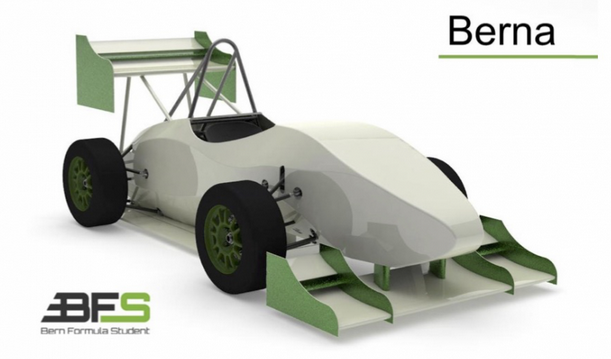
\includegraphics[width=150mm]{bilder/berna.png}			% Titelbild definieren
\end{textblock}

\begin{textblock}{154}(28,135)
	\begin{picture}(150,2)
		\put(0,0){\color{bfhgrey}\rule{150mm}{2mm}}
	\end{picture}
\end{textblock}
\color{black}

% Institution / Titel / Untertitel / Autoren / Experten:
%---------------------------------------------------------------------------
\begin{flushleft}

\vspace*{115mm}

\fontsize{26pt}{28pt}\selectfont 
\titel 				\\							% Titel aus der Datei vorspann/titel.tex lesen
\vspace{2mm}

%\fontsize{16pt}{20pt}\selectfont\vspace{0.3em}
%Hier steht ein Untertitel 			\\							% Untertitel eingeben
\vspace{5mm}

\fontsize{10pt}{12pt}\selectfont
\textbf{Semesterarbeit im Rahmen des Modules Projekt 2} \\									% eingeben
\vspace{3mm}

% Abstract (eingeben):
%---------------------------------------------------------------------------
%\begin{textblock}{150}(28,190)
%\fontsize{10pt}{12pt}\selectfont
%[Kurztext (Abstract) einfügen, falls gewünscht] \\ 
%Dieses Dokument dient als Vorlage für die Erstellung von Berichten nach den Richtlinien der BFH. Die %Vorlage ist in \LaTeX{} erstellt und unterstützt das automatische Erstellen von diversen %Verzeichnissen, Literaturangaben, Indexierung und Glossaren. Dieser kleine Text ist eine %Zusammenfassung über das vorliegenden Dokument mit einer Länge von 4 bis max. 8 Zeilen. \\
%Das Titelbild kann in den Zeilen 157/158 der Datei template.tex ein- oder ausgeschaltet werden.
%\end{textblock}

\begin{textblock}{150}(28,225)
\fontsize{10pt}{17pt}\selectfont
\begin{tabbing}
xxxxxxxxxxxxxxx\=xxxxxxxxxxxxxxxxxxxxxxxxxxxxxxxxxxxxxxxxxxxxxxx \kill
Studiengang:	\> Informatik	\\			% Namen eingeben
Autoren:		\> Pascal Bohni, Roger Jaggi		\\					% Namen eingeben
Betreuer:	\> Dr.~Andreas Danuser		\\					% Namen eingeben
%Auftraggeber:	\> [Wwwww AG]						\\					% Namen eingeben
%Experten:		\> [Dr.~Zzzz Zzzz]				\\					% Namen eingeben
Datum:			\> \versiondate					\\		% aus Datei vorspann/version.tex lesen
\end{tabbing}

\end{textblock}
\end{flushleft}

\begin{textblock}{150}(28,280)
\noindent 
\color{bfhgrey}\fontsize{9pt}{10pt}\selectfont
Berner Fachhochschule | Haute école spécialisée bernoise | Bern University of Applied Sciences
\color{black}\selectfont
\end{textblock}


\end{titlepage}

%
% ===========================================================================
% EOF
%
			% activate for Titelseite mit Bild
% Versionenkontrolle :
% -----------------------------------------------
Das Bild von der Titelseite entstammt der Website der Bern Formula Student, erreichbar unter http://www.bernformulastudent.ch

\begin{textblock}{180}(15,150)
\color{black}
\begin{huge}
Versionen
\end{huge}
\vspace{10mm}

\fontsize{10pt}{18pt}\selectfont
\begin{tabbing}
xxxxxxxxxxx\=xxxxxxxxxxxxxxx\=xxxxxxxxxxxxxx\=xxxxxxxxxxxxxxxxxxxxxxxxxxxxxxxxxxxxxxxxxxxxxxx \kill
Version	\> Datum	\> Status		\> Bemerkungen		\\
0.1	\> 01.08.2013	\> Entwurf		\> Lorem ipsum dolor sit amet	\\	
0.2	\> 21.08.2013	\> Entwurf		\> Phasellus scelerisque	\\ 
0.3	\> 02.09.2013	\> Entwurf		\> Donec eget aliquam urna. Lorem ipsum dolor sit amet	\\ 
1.0	\> 12.09.2013	\> Definitiv	\> Lorem ipsum dolor sit ametPhasellus scelerisque, leo sed iaculis ornare 	\\ 
1.1	\> 04.11.2013	\> Korrektur	\> Layout angepasst	\\
1.2	\> 01.02.2014	\> Ergänzung	\> Kapitel 1.1 erweitert	\\
\end{tabbing}

\end{textblock}

\color{black}
\cleardoubleemptypage
\setcounter{page}{1}
\cleardoublepage
\phantomsection 
\addcontentsline{toc}{chapter}{Management Summary}
\chapter*{Management Summary}
\label{chap:managementSummary}

Lorem ipsum dolor sit amet, consectetur adipiscing elit. Phasellus scelerisque, leo sed iaculis ornare, mi leo semper urna, ac elementum libero est at risus. Donec eget aliquam urna. Lorem ipsum dolor sit amet, consectetur adipiscing elit. Nunc fermentum nunc sollicitudin leo porttitor volutpat. Duis ac enim lectus, quis malesuada lectus. Aenean vestibulum suscipit justo, in suscipit augue venenatis a. Donec interdum nibh ligula. Aliquam vitae dui a odio cursus interdum quis vitae mi. Phasellus ornare tortor fringilla velit accumsan quis tincidunt magna eleifend. Praesent nisl nibh, cursus in mattis ac, ultrices ac nulla. Nulla ante urna, aliquet eu tempus ut, feugiat id nisl. Nunc sit amet mauris vitae turpis scelerisque mattis et sed metus. Aliquam interdum congue odio, sed semper elit ullamcorper vitae. Morbi orci elit, feugiat vel hendrerit nec, sollicitudin non massa. Quisque lacus metus, vulputate id ullamcorper id, consequat eget orci \nocite{kopka:band1} \nocite{Marti06}. 

\cleardoubleemptypage
%---------------------------------------------------------------------------

% Table of contents
%---------------------------------------------------------------------------
\tableofcontents
\cleardoublepage
%---------------------------------------------------------------------------

% Main part:
%---------------------------------------------------------------------------
\pagenumbering{arabic}

\chapter{Aufgabenstellung}
\label{chap:aufgabenstellung}

Von Seiten Bern Formula Student wurde folgende Zielvorstellung an die Telemetrie formuliert:

\textit{Grundsätzliches möglichst alle Daten übermitteln, die auf den drei CAN-Bus-Systemen des Fahrzeuges übertragen werden.} 

Zum jetzigen Zeitpunkt sind dies:

\begin{itemize}
	\itemsep 1pt \parskip 0pt \parsep 0pt
	\item \textbf{Eingangsgrössen Fahrer}		
		\begin{itemize}
			\itemsep 1pt \parskip 0pt \parsep 0pt
			\item Fahrpedalstellung		\textit{CAN 1}
			\item Bremspedalstellung	\textit{CAN 1}
			\item Bremsdruck			\textit{CAN 1}
			\item Lenkwinkel			\textit{CAN 1}
		\end{itemize}
	\item \textbf{Motor und Kühlsystem}		
		\begin{itemize}
			\itemsep 1pt \parskip 0pt \parsep 0pt
			\item Soll-Moment			\textit{CAN 2/3}
			\item Ist-Moment			\textit{CAN 2/3}
			\item Soll-Drehzahl			\textit{CAN 2/3}
			\item Ist-Drehzahl			\textit{CAN 2/3}
			\item Motortemperatur		\textit{CAN 2/3}
			\item Kühlmitteltemperatur	\textit{CAN 1}
		\end{itemize}		
	\item \textbf{Batterie}		
		\begin{itemize}
			\itemsep 1pt \parskip 0pt \parsep 0pt
			\item HV-Spannung				\textit{CAN 1}
			\item HV-Stromg					\textit{CAN 1}
			\item HV-Batterie Ladestand		\textit{CAN 1}
			\item GLV Batterie Spannung		\textit{Wireless über Sming}
		\end{itemize}
					
	\item \textbf{Fahrzeug}		
	\begin{itemize}
		\itemsep 1pt \parskip 0pt \parsep 0pt
		\item Geschwindigkeit						\textit{CAN 1}
		\item Beschleunigung						\textit{CAN 1}
		\item Drehrate 								\textit{CAN 1}
		\item Reifentemperatur						\textit{Wireless über Sming}
		\item Bremstemperatur						\textit{Wireless über Sming}
		\item Bodentemperatur						\textit{Wireless über Sming}
		\item Lufttempertur bei Kühlereintritt		\textit{Wireless über Sming}
		\item Lufttempertur bei Kühleraustritt		\textit{Wireless über Sming}
		\item Dämpferweg (optional)					\textit{Wireless über Sming}
		
	\end{itemize}			
\end{itemize}

Die Anbindung "Wireless über Sming" bedeutet, dass wir selber Sensoren zur Erfassung der gewünschten Messgrössen liefern sollen. Die Sensoren sollen dabei drahtlos über den Bluetooth-Stack des Smings kommunizieren.

Erweitert wurde die Aufgabenstellung von Andreas Danuser durch die Konstruktionsvorgabe, dass die einzelnen Komponenten der Telemetrie möglichst universell, sprich als eigenständiges Modul auch in einem komplett anderen Einsatzzweck, verwendbar sein sollen.


\chapter{Aufbau}
\label{chap:aufbau}

Anhand der Aufgabenstellung wurde eine Architektur entworfen, die aus mehreren Modulen besteht. Die einzelnen Module werden in den nächsten Kapiteln beschrieben. Die Abbildung \ref{fig:gesamtarchitektur_telemetrie} zeigt die gewählte Architektur.


\begin{figure}[hbtp]
    \center
    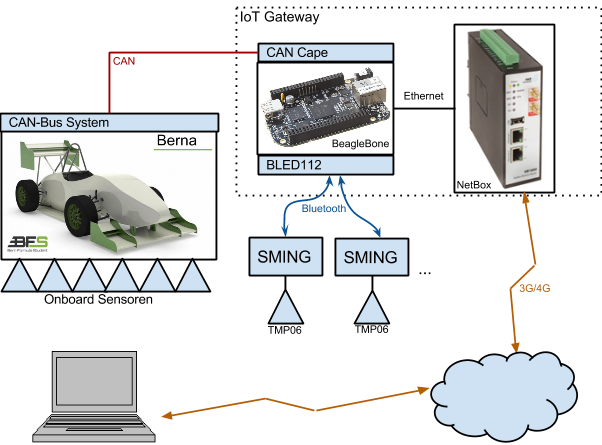
\includegraphics[width=\textwidth]{bilder/gesamtarchitektur.png}
    \caption{Gesamtarchitektur Telemetrie}
    \label{fig:gesamtarchitektur_telemetrie}
\end{figure}


\chapter{IoT Gateway}\label{chap:iotgateway}

Das IoT Gateway dient dazu einzelne Messpunkte zusammen zufassen und die Daten danach ins Internet zu übertragen. Als Gateway Hardware nutzen wir die bekannte Embedded Platform Beagle Bone Black. Dies ermöglicht uns auch vorhandene Erweiterungen zu nutzen. Das Gateway arbeitet mit zwei verschiedenen Methoden um die einzelnen Messpunkte abfragen zu können. Einerseits dem CAN-Bus, welcher in der Automobiltechnik sehr verbreitet ist und anderseits eine Bluetooth Smart Schnittstelle um die Sming Messknoten ansprechen zu können. Die Übertragung ins Internet wird mithilfe eines UMTS-Routers gemacht.


%Unser Internet of Things Gateway besteht wiederum aus mehreren Teilen. Die einzelnen Sensoren werden entweder über den CAN-Bus oder an ein Sming angeschlossen. Der CAN-Bus wird von uns über ein BeagleBone Cape mitgelesen. Die Daten des Smings können wir ebenfalls auf dem BeagleBone empfangen. Dies erreichen wir mit Hilfe des Bluetooth Smart USB Dongle BLED112 von Bluegiga, welcher am BeagleBone angeschlossen wird.

\begin{figure}[hbtp]
    \center
    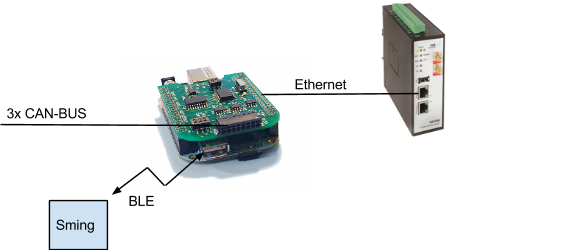
\includegraphics[width=\textwidth]{bilder/aufbau_in_auto.png}
    \caption{Aufbau des IoT Gateways}
    \label{fig:aufbau_iot_gateway}
\end{figure}

\section{Netmodule NetBox NB1600}\label{sec:netbox}
Als UMTS-Router setzen wir auf den Netmodule Router NB1600. Dieser kam schon in unserem Schwerpunkt Mobile Computing beim Semesterprojekt "Smoje" zum Einsatz. Für unseren Einsatzzweck als reine Bridge zwischen Ethernet und UMTS-Netz wird er nicht ausgelastet. Der NB1600 könnte nähmlich auch noch GPS empfangen und als Wlan-Hotspot dienen. Daher besteht hier noch eine Optimierungsmöglichkeit durch den Einsatz eines geigneten USB Dongles der direkt vom Beagle Bone aus auf UMTS zugreifen kann. Dieser zu evaluieren hätte aber den Zeitrahmen für das Projekt gesprengt.

\begin{figure}[hbtp]
	\center
	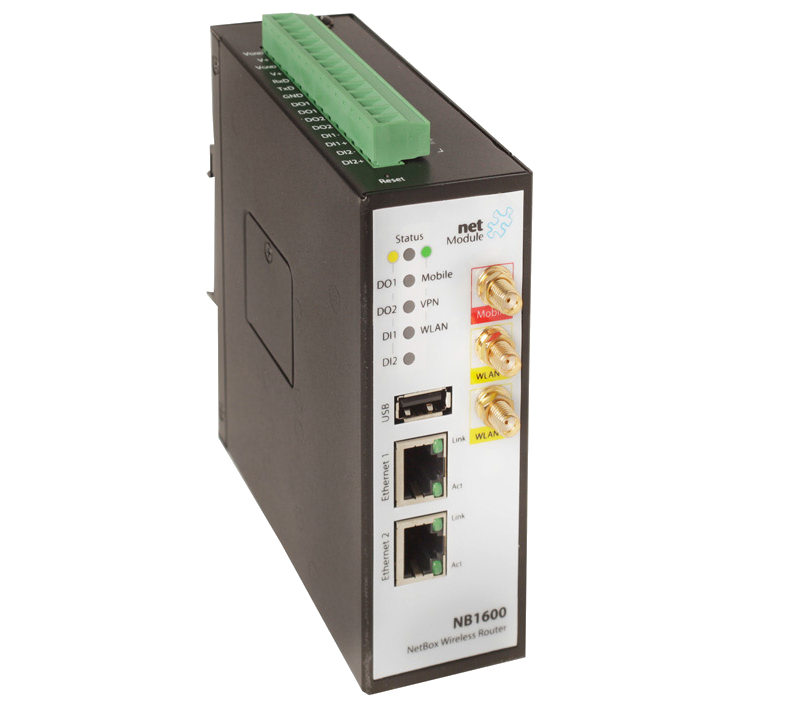
\includegraphics[width=6cm]{bilder/netmodule.png}
	\caption{Foto NetModule NB1600}
	\label{fig:netbox}
\end{figure}


\section{CAN-Cape}
%Als Basis für unsere Software kommt ein BeagleBone Black als Recheneinheit zum Einsatz. Zum Anschliessen der drei CAN-Busse des Fahrzeuges verwenden wir ein von einem Italiener gefertigtes CAN-Cape, dass einfach auf das Beaglebone drauf gesteckt werden kann:

 Der CAN-Bus wird im Bern Formula Student Projekt genutzt um die Steuerbefehle innerhalb des Autos zu übertragen. Es werden drei seperate Verdrathungen geführt. Wir empfangen die Daten der 3 CAN-Busse über das Beagle Bone Black CAN Cape von Tower Tech. Da die ganze Steuerung des Autos über die CAN-Busse läuft haben wir nur lesenden Zugriff. Die Installationsanleitung zum Cape befindet sich im Anhang.

\begin{figure}[hbtp]
	\center
	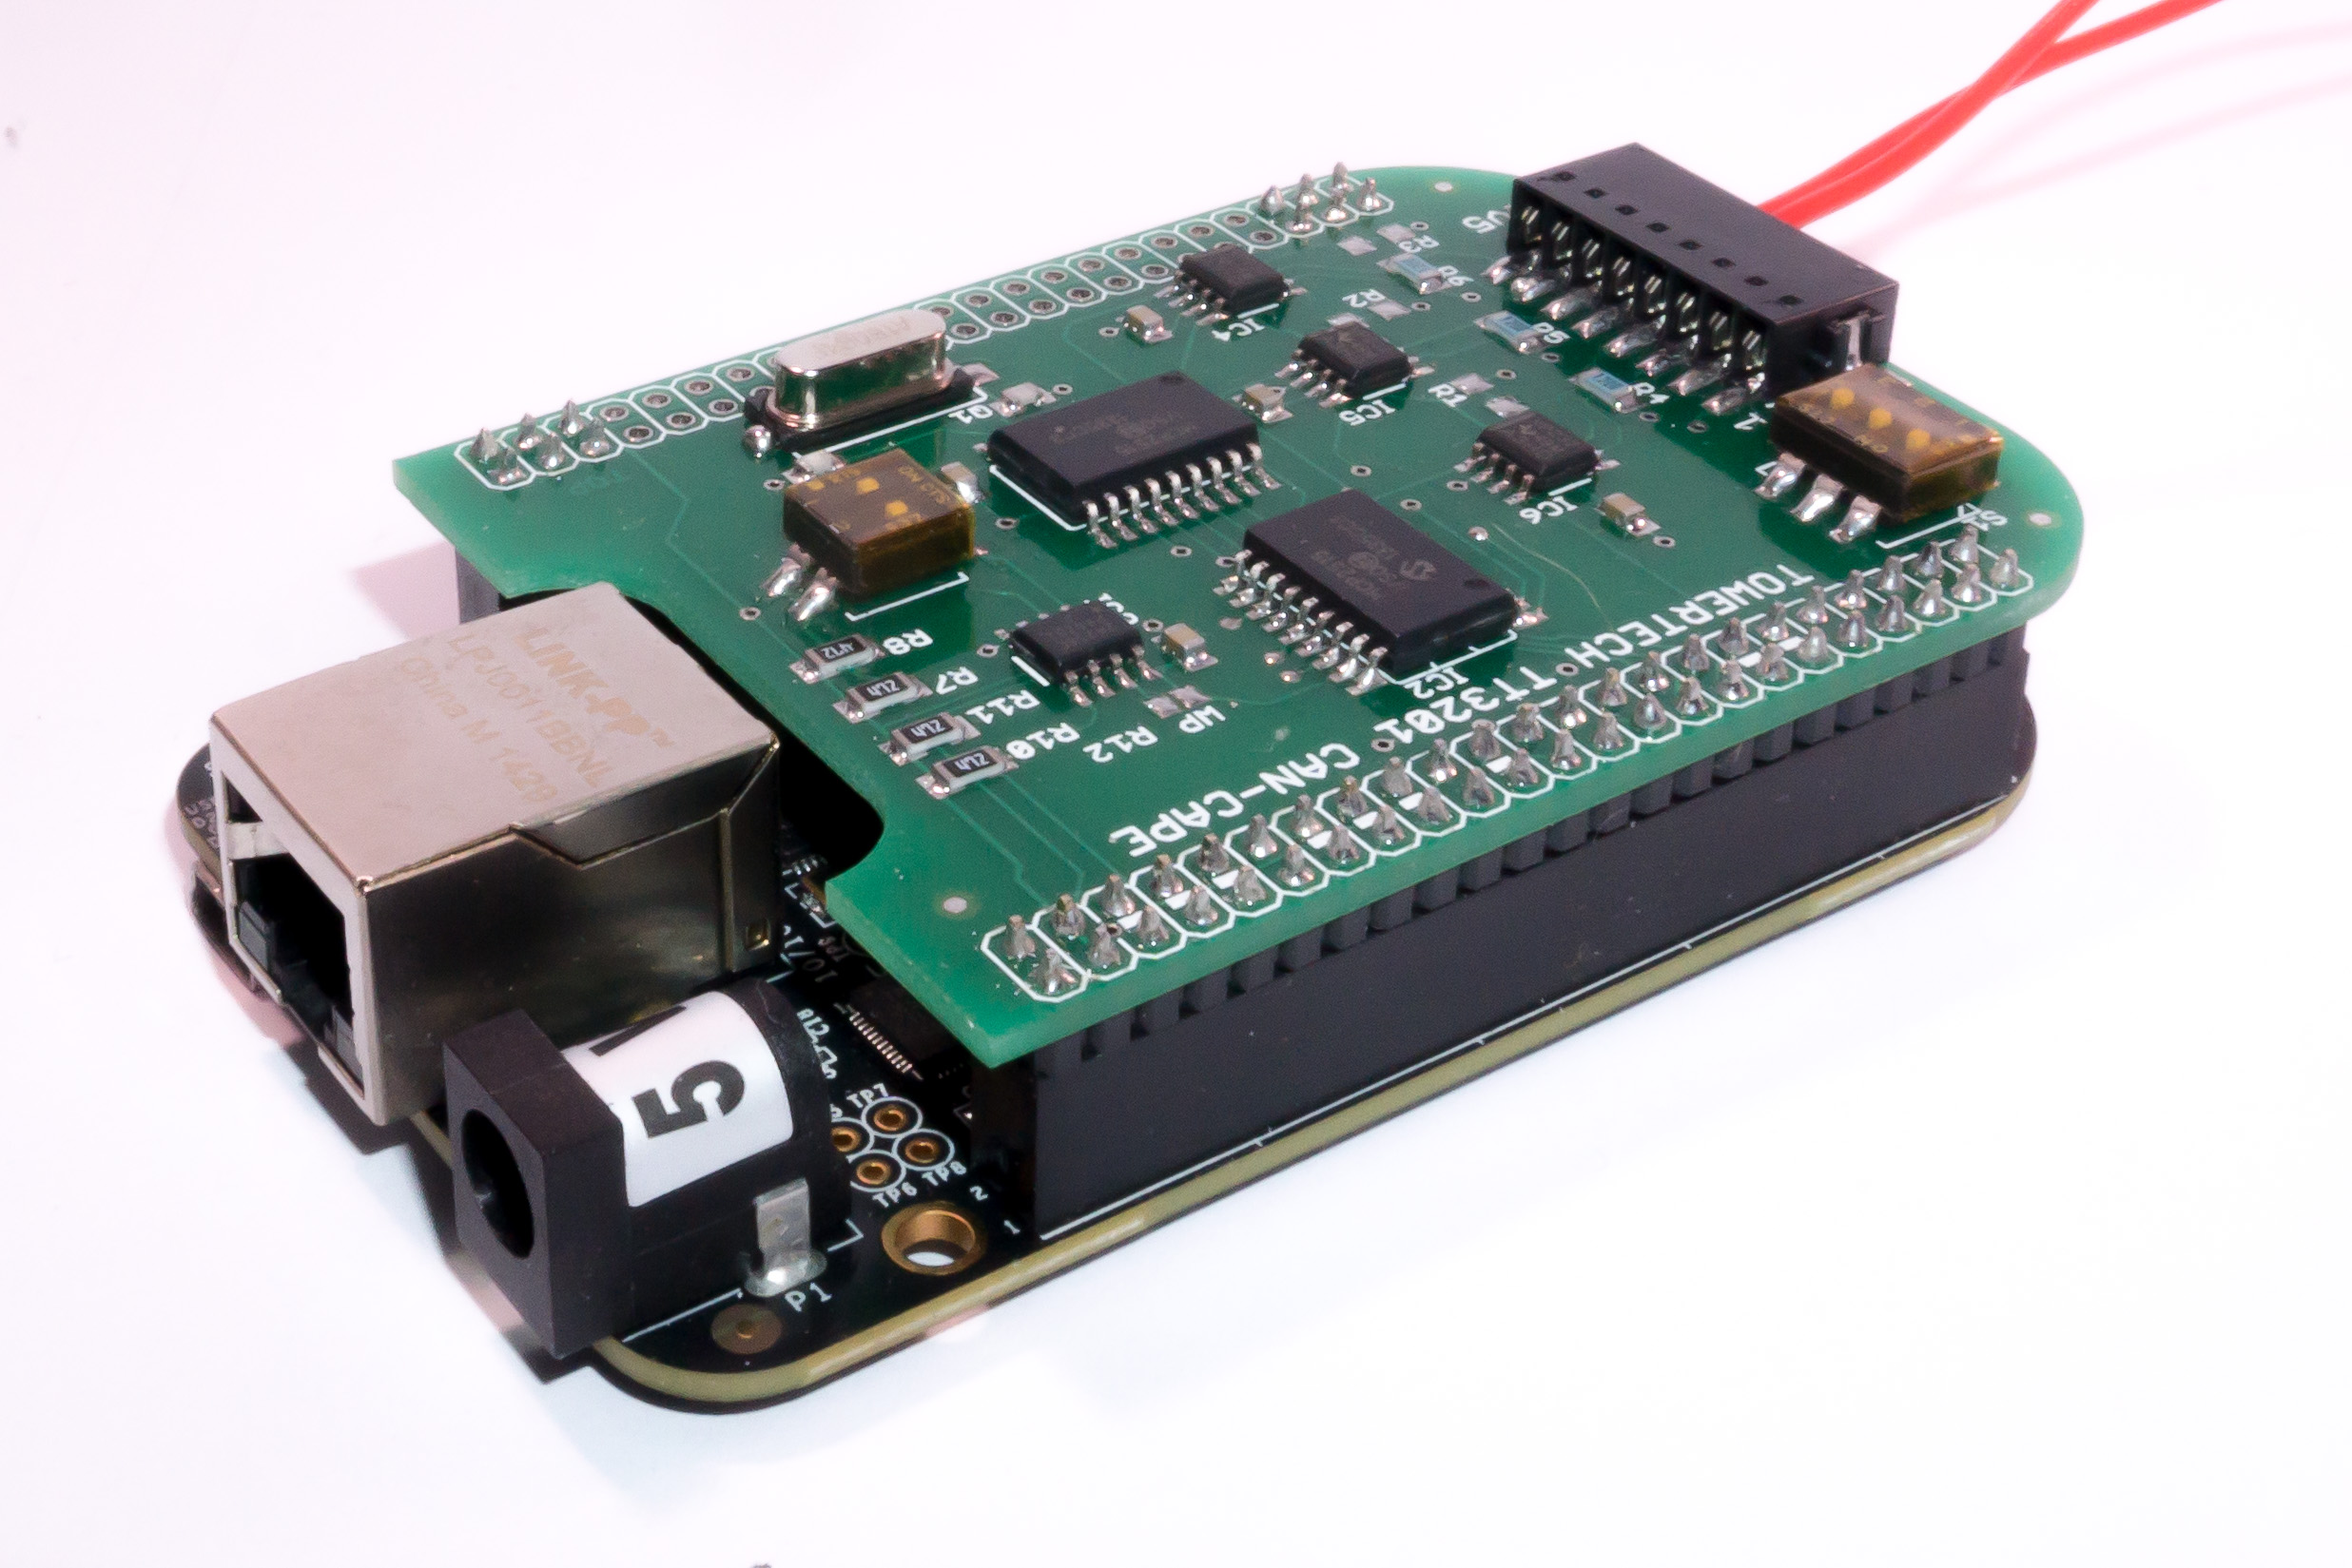
\includegraphics[width=\textwidth]{bilder/foto-4.jpg}
	\caption{Foto CanCape auf Bealge Bone Black}
	\label{fig:CanCape}
\end{figure}

%\textbf{Installationsinstruktionen siehe Anhang.}



\section{BLED112}
Die zweite Schnittstelle zu den Sensoren ist der USB Dongle BLED112 von Bluegiga. Dieser integriert den ganzen Bluetooth Smart Stack, der dank einer API über eine serielle Schnittstelle angesprochen werden kann.

\begin{figure}[hbtp]
	\center
	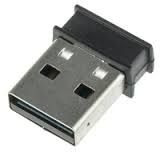
\includegraphics[width=4cm]{bilder/bled112.jpg}
	\caption{Foto BLED112}
	\label{fig:bled112}
\end{figure}

Die wichtigsten zu wissenden Details über den Bluegiga Dongle sind die folgenden:

\begin{itemize}
\itemsep 1pt \parskip 0pt \parsep 0pt
\item Kommunikation erfolgt über serielle Schnittstelle. Dem BLED112 werden darüber einfach die enstprechenden Anweisungen gesendet.

\item Material zu BLED112 (API Doku, Windows Treiber, Linux/Mac works out of the box) \url{https://www.bluegiga.com/en-US/products/bled112-bluetooth-smart-dongle/#documentation} → siehe im Speziellen API 1.3 Referenz


\item Java-LIB, wo die BLED 112 API bereits implementiert ist: \url{https://github.com/SINTEF-9012/bglib}


\item Ein paar Worte zum BLED112 selber:
	\begin{itemize}
	\itemsep 1pt \parskip 0pt \parsep 0pt
	\item  Das Teil ist programmierbarer Mikrocontroller mit komplett implementiertem Bluetooth-Stack, verpackt als USB-Dongle (Dongle = das D im BLED112)

	\item  Durch die Programmierung in Bluescript kann der Dongle unter anderem zu einem iBeacon gemacht werden.


	\item  Theoretisch bietet er aber viel mehr an. Er ist nebenbei ein direktes Konkurrenzprodukt zum nRF51 Chip von Nordic, der auf dem Sming zum Einsatz kommt.
	\end{itemize}


\item Beispiel-Befehlsabfolge, wie sie beim Sming zum Einsatz kommt. Detailbeschrieb der Parameter siehe Bluegiga API 1.3 Doku. Die Parameter-Werte entsprechen denen im Demo-Script und sollten lauffähig sein:

	\begin{itemize}
	\itemsep 1pt \parskip 0pt \parsep 0pt
	\item Suche nach BLE Advertisments
		\begin{itemize}
			\itemsep 1pt \parskip 0pt \parsep 0pt
			\item bg.api.gapSetScanParameters(0xC8, 0xC8, 0)
			\item bg.api.gapDiscover(1)
		\end{itemize}

	\item Wenn ein Device mit Name TXW51 gefunden, beende Suche kommt als Event mit Class = GenericAccessProfile siehe Demo-Script ab Zeile 238
		\begin{itemize}
			\itemsep 1pt \parskip 0pt \parsep 0pt
			\item Suche beenden: bg.api.gapEndProcedure()
		\end{itemize}
	

	\item Verbinde zum gefundenen Device anhand seiner MAC-Adresse
		\begin{itemize}
			\itemsep 1pt \parskip 0pt \parsep 0pt
			\item bg.api.gapConnectDirect( <MAC-Addr>, 1, 60, 76, 100, 9)
		\end{itemize}



	\item Hole einfach mal komplette Handle-Liste der Bluetooth Attribute (Optimieriungspotential da)
			\begin{itemize}
				\itemsep 1pt \parskip 0pt \parsep 0pt
				\item bg.api.attClientFindInformation( <connectionHandle>, 1, 0xffff)
			\end{itemize}


	\item Stimme die SMING UUIDs mit denen in der Handle-Liste überein. Merke zu jeder UUID deren Handle sowie UUID der CCID Attributes (siehe später)


	\item Lese mit den entsprechenden Handle das Attribut (ich habe einfach mal jeweils immmer gerade mal alle eingelesen)
			\begin{itemize}
				\itemsep 1pt \parskip 0pt \parsep 0pt
				\item bg.api.attClientReadByHandle(<connection>, <uuid handle> )
			\end{itemize}


	\item Zum Aktivieren der Accelometer-Messungen müssen folgende Attributte geschrieben werden:
			\begin{itemize}
				\itemsep 1pt \parskip 0pt \parsep 0pt
				\item bg.api.attClientAttributeWrite( <connection>, <uuid handle>, <newValue>)
				\item \url{LSM330_CHAR_GYRO_EN} = 1 
				\item \url{LSM330_CHAR_ACC_EN} = 1 
				\item \url{CCID UUID 0x02, 0x29 = 0x01, 0x00} ( Dies aktiviert das Bluetooth Feature CCID, wodruch das Sming bei Sming seitiger Attributwertänderung automatisch den neuen Wert sendet. Die Messwerte werden so per Push übertragen. Seitens Sming wird somit einfach der Messwert auf das Attribut \url{MEASURE_CHAR_DATASTREAM} geschrieben. Dies löst aus, dass der Bluetooth Stack des Smings automatisch den neue Messwert als Event zum Bluegiga Dongle übertragt und wir das so mitkriegen)
				\item \url{MEASURE_CHAR_START} = 1
			\end{itemize}


	\item Das Lesen der Temperatur muss mit einem Polling auf Attribut \url{LSM330_CHAR_TEMP_SAMPLE} gemacht werden.

	\item Beende Verbindung zum Sming
			\begin{itemize}
				\itemsep 1pt \parskip 0pt \parsep 0pt
				\item bg.api.connectionDisconnect( <connection> )
			\end{itemize}
	\end{itemize}
\end{itemize}

\chapter{SMING}\label{sec:sming}
Um weitere Sensoren einfach ohne Verdrahtung ins Messsystem aufzunehmen, setzen wir auf das Sming. Das Sming wurde durch Daniel Meer in seiner Master Thesis entwickelt. Er beschreibt in der Thesis das Sming wie folgt: \textit{Der TXW51 ist ein kleiner und energiesparender Sensorknoten, der als Basis für zukünftige Projekte verwendet werden kann. Er kommuniziert über Bluetooth Smart und enthält einen Sensor zur Messung der Beschleunigung. Die Firmware kann einfach für neue Anforderungen modifiziert werden.}\cite{meer:masterthesis}

\begin{figure}[hbtp]
	\center
	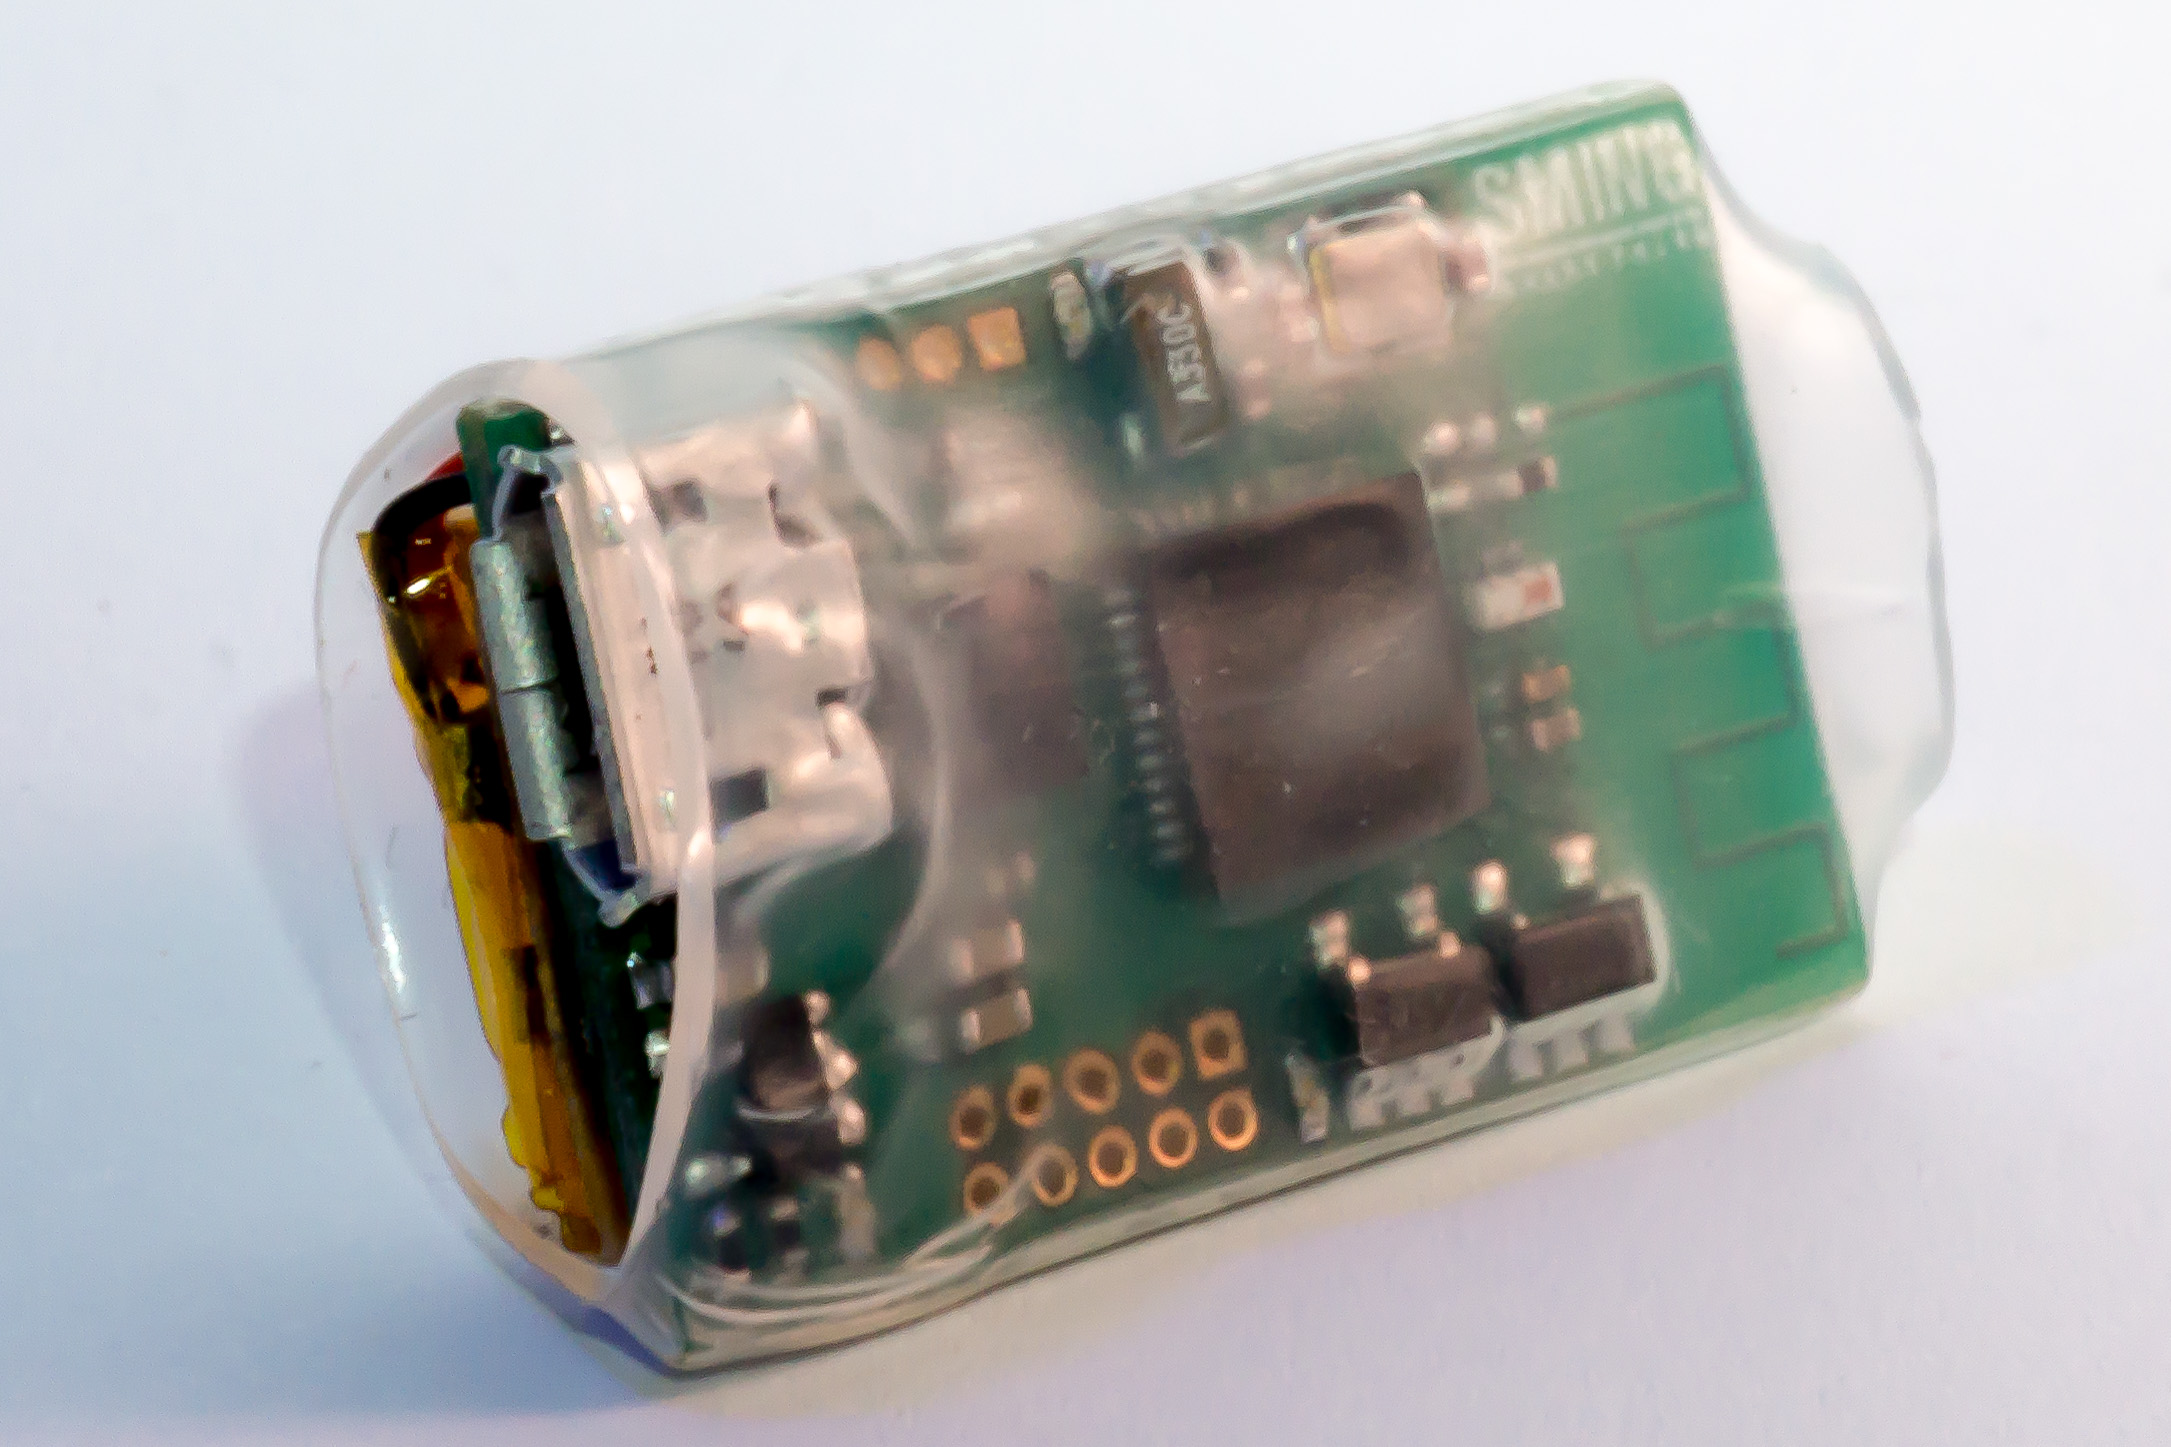
\includegraphics[width=10cm]{bilder/foto-6.jpg}
	\caption{Foto Sming mit Akku bestückt}
	\label{fig:sming}
\end{figure}

Für unser Projekt ist vorallem die Erweiterbarkeit des Sming sehr interessant. Dies weil beliebige Senosoren über I2C angesprochen werden können.

Hier nochmals die wichtigsten Eigenschaften:

\begin{itemize}
	\itemsep 1pt \parskip 0pt \parsep 0pt
	\item Kommunikation über Bluetooth 4.0
	\item Werte werden über BLE GATT gelesen und geschrieben 
	\item Speziell wissenswert: Messungen werden per PUSH über Bluetooth CCID Feature gesendet, Details siehe Beschreibung BLED112
	\item Bluetooth Device Name ist bei allen Smings von der BFH Burgdorf:  TXW51
	\item Grundsätzlich sind die Attribute des SMINGS in drei Gruppen unterteilbar:
	\begin{itemize}
		\itemsep 1pt \parskip 0pt \parsep 0pt
		\item Beginnend mit \url{DEVICE_INFO}: diverse einfache Textfelder, die auch selber nach gutdünken beschrieben werden können.
		\item Beginnend mit LSM330: Die entsprechenden Einstellung und Werte des LSM330-Sensors (Kombinierter Gyro-,Accelometer- und Temperatur-Sensor)
		\item Beginnend mit MEASURE: Die entsprechenden Funktionen, um die asynchrone Messung via Bluetooth Push zu konfigurieren (Dauer), zu starten, zu stoppen und auch von Hand den letzten Messwert abzufragen.
		
	\end{itemize}
	\item Tipp: Über das Demo-Tool von Bluegiga kann händisch mit dem SMING verbunden und Attribute gelesen/geschrieben werden.
	
	\item Messwert-Attribut: Zum Optimieren der Performance sind auf dem Messwert-Attribut oft bis zu drei Messwerte binär aneinandergereit vorhanden. Das Decodieren des Wertes wird im Demo-Script von Zeile 319 bis 345 gemacht.
	
	\item Java-Beispielcode für Kommunikation ist ebenfalls vorhanden,siehe gezippter Source der Demo-Android App von Daniel Meer auf Google Drive. Dort wird aber mit den Android Bluetooth Stack gearbeitet und nicht mit dem Bluegiga, weswegen sich das leider nicht ganz eins zu eins kopieren lässt. 
	
	\item Hinweis: das CCID wird von Android im Gegensatz zu Bluegiga als Funktion abstrahiert.
\end{itemize}

\subsection{Liste der wichtigsten Attribut UUIDs}
\begin{lstlisting}
DEVICE_INFO_SERVICE           : "8EDF0100-67E5-DB83-F85B-A1E2AB1C9E7A",
DEVICE_INFO_CHAR_MANUFACTURER : "8EDF0101-67E5-DB83-F85B-A1E2AB1C9E7A",
DEVICE_INFO_CHAR_MODEL        : "8EDF0102-67E5-DB83-F85B-A1E2AB1C9E7A",
DEVICE_INFO_CHAR_SERIAL       : "8EDF0103-67E5-DB83-F85B-A1E2AB1C9E7A",
DEVICE_INFO_CHAR_HW_REV       : "8EDF0104-67E5-DB83-F85B-A1E2AB1C9E7A",
DEVICE_INFO_CHAR_FW_REV       : "8EDF0105-67E5-DB83-F85B-A1E2AB1C9E7A",
DEVICE_INFO_CHAR_DEVICE_NAME  : "8EDF0106-67E5-DB83-F85B-A1E2AB1C9E7A",
DEVICE_INFO_CHAR_SAVE_VALUES  : "8EDF0107-67E5-DB83-F85B-A1E2AB1C9E7A",

LSM330_SERVICE           : "8EDF0200-67E5-DB83-F85B-A1E2AB1C9E7A",
LSM330_CHAR_ACC_EN       : "8EDF0201-67E5-DB83-F85B-A1E2AB1C9E7A",
LSM330_CHAR_GYRO_EN      : "8EDF0202-67E5-DB83-F85B-A1E2AB1C9E7A",
LSM330_CHAR_TEMP_SAMPLE  : "8EDF0203-67E5-DB83-F85B-A1E2AB1C9E7A",
LSM330_CHAR_ACC_FSCALE   : "8EDF0204-67E5-DB83-F85B-A1E2AB1C9E7A",
LSM330_CHAR_GYRO_FSCALE  : "8EDF0205-67E5-DB83-F85B-A1E2AB1C9E7A",
LSM330_CHAR_ACC_ODR      : "8EDF0206-67E5-DB83-F85B-A1E2AB1C9E7A",
LSM330_CHAR_GYRO_ODR     : "8EDF0207-67E5-DB83-F85B-A1E2AB1C9E7A",
LSM330_CHAR_TRIGGER_VAL  : "8EDF0208-67E5-DB83-F85B-A1E2AB1C9E7A",
LSM330_CHAR_TRIGGER_AXIS : "8EDF0209-67E5-DB83-F85B-A1E2AB1C9E7A",

MEASURE_SERVICE         : "8EDF0300-67E5-DB83-F85B-A1E2AB1C9E7A",
MEASURE_CHAR_START      : "8EDF0301-67E5-DB83-F85B-A1E2AB1C9E7A",
MEASURE_CHAR_STOP       : "8EDF0302-67E5-DB83-F85B-A1E2AB1C9E7A",
MEASURE_CHAR_DURATION   : "8EDF0303-67E5-DB83-F85B-A1E2AB1C9E7A",
MEASURE_CHAR_DATASTREAM : "8EDF0304-67E5-DB83-F85B-A1E2AB1C9E7A"
\end{lstlisting}

\section{BLE-I2C Bridge}
\label{bleI2cBridge}

Das Sming verfügt über den Erweiterungsheader die Möglichkeit I2C Sensoren anzusprechen. Um diese Funktion zu nutzen muss die Firmware des Smings erweitert werden. Dies ist nicht Straight-Forward weil für die Entwicklung in C und das Deployment auf den NRF51 spezielle Hardware und Software erforderlich ist. Um dieses Problem zu umgehen wurde die BLE-I2C Bridge entwickelt. Sie soll dazu dienen, dass vom IoT-Gateway via Sming I2C Sensoren und Aktoren angesprochen werden können. Somit muss für einen neuen Sensor die Firmware der Smings nicht angerührt werden. Dafür muss aber das IoT-Gateway programmiert werden. Dieses lässt sich aber je nach Gateway Typ leicht über Ethernet oder USB programmieren. Auch die Softwareentwicklung in JavaScript sollte denn meisten Entwickler in der Informatik Branche weniger schwer fallen als dies bei C der Fall ist.

\begin{figure}[hbtp]
    \center
    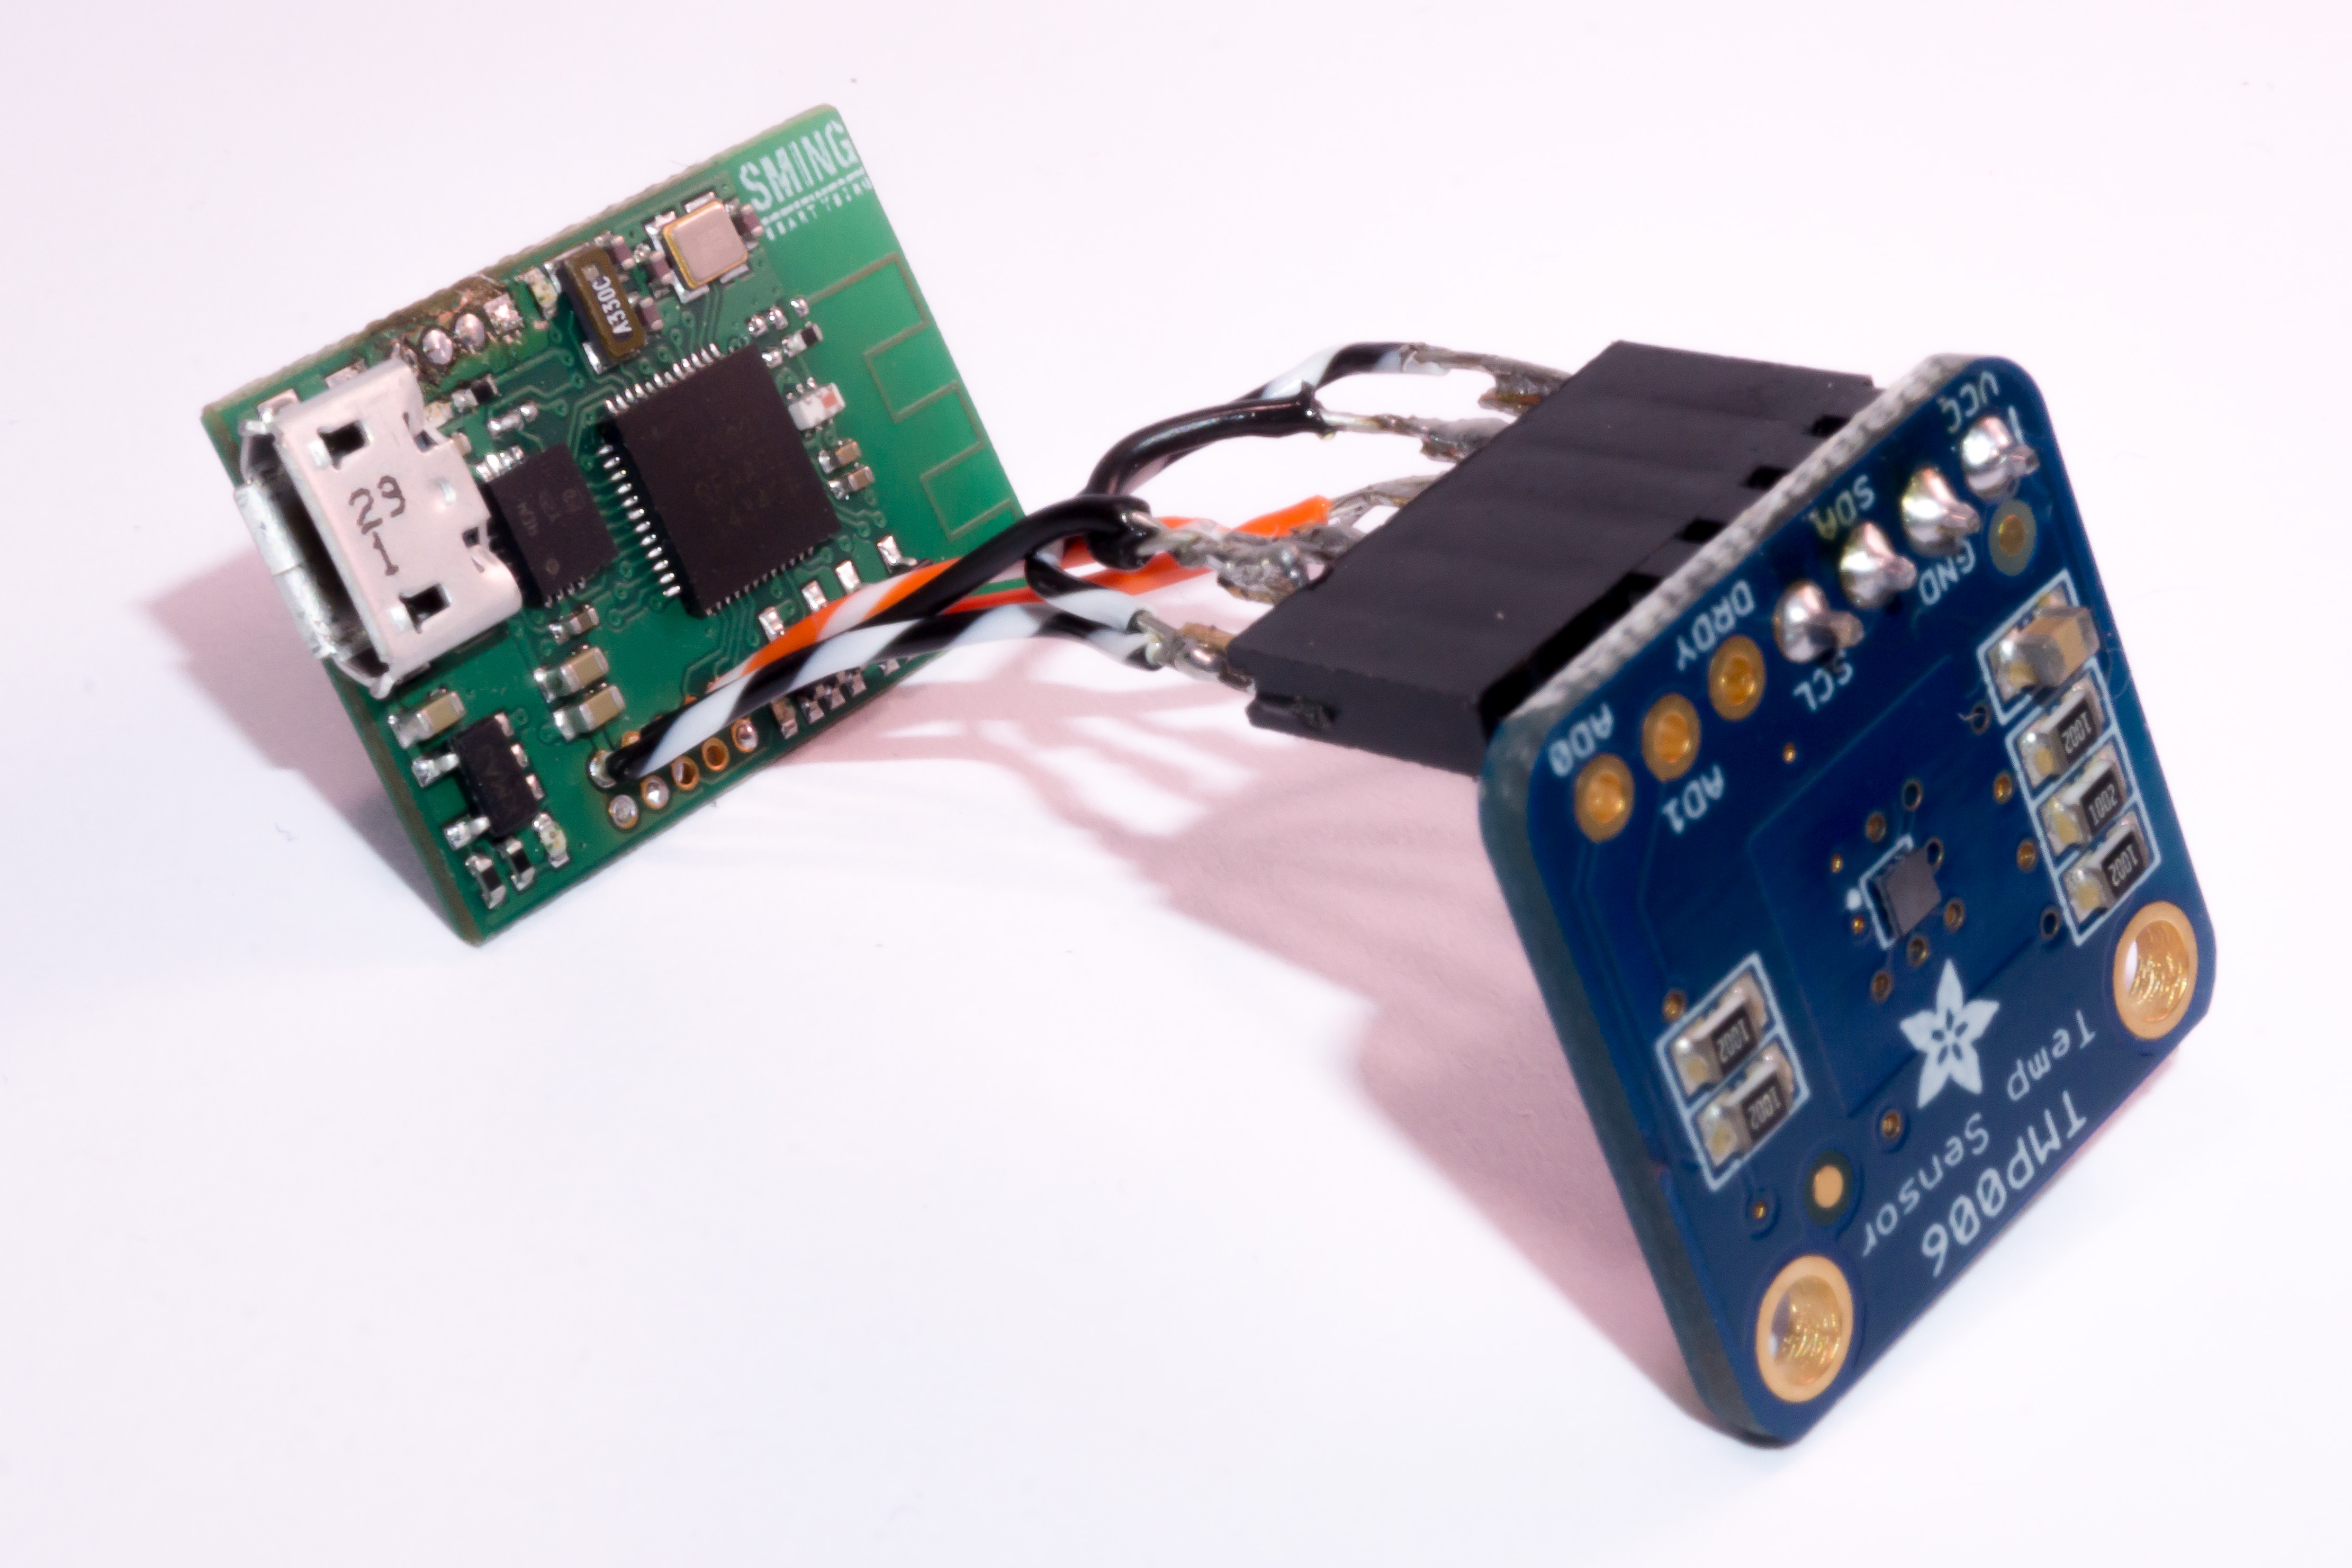
\includegraphics[width=\textwidth]{bilder/foto-2.jpg}
    \caption{Sming mit über I2C Bridge abfragbaren TMP06 Sensor}
    \label{fig:sming_mit_tmp06}
\end{figure}


\section{Implementation}
\label{bleI2cImplementation}

Für die BLE-I2C Bridge wurde ein eigener BLE-Service aufgesetzt.

%\begin{table}[h]
%\centering
\begin{tabularx}{\textwidth}{|l|X|}
\hline
Name & I2C Service                                       \\
\hline
Beschreibung & Ein Service für I2C Devices über BLE anzusprechen \\
\hline
UUID	&    0x8EDF0500-67E5-DB83-F85B-A1E2AB1C9E7A  \\
\hline                                            
\end{tabularx}
%\caption{Ble I2C Service}
%\label{tab:bleI2cService}
%\end{table}

folgende Charakteristiken stehen bei diesem Service zur Verfügung:

%\begin{table}[h]
%\centering
\begin{tabularx}{\textwidth}{|l|X|}
\hline
Name & I2C Device Adress                                   \\
\hline
Beschreibung & Wird verwendet um die I2C Adresse des Sensor (oder Aktor) im Sming einzustellen. \\
\hline
UUID	&    0x8EDF0501-67E5-DB83-F85B-A1E2AB1C9E7A  \\
\hline     
Anzahl Byte	&    1  \\
\hline      
Zugriffsrechte	&   R/W  \\
\hline        
Wertebereich	&   0x00 .. 0x7F \\
\hline          
Wertebereich	&   0x00 \\
\hline                                     
\end{tabularx}
%\caption{Ble I2C Device Adress Charakteristik}
%\label{tab:bleI2cDeviceAdress}
%\end{table}

%\begin{table}[h]
%\centering
\begin{tabularx}{\textwidth}{|l|X|}
\hline
Name & I2C Device Register                                  \\
\hline
Beschreibung & Wird verwendet um das I2C Register des Sensor (oder Aktor) im Sming einzustellen, auf welches geschrieben oder von welchem gelesen werden soll. \\
\hline
UUID	&    0x8EDF0502-67E5-DB83-F85B-A1E2AB1C9E7A  \\
\hline     
Anzahl Byte	&    1  \\
\hline      
Zugriffsrechte	&   R/W  \\
\hline        
Wertebereich	&   0x00 .. 0xFF \\
\hline          
Wertebereich	&   0x00 \\
\hline                                     
\end{tabularx}
%\caption{Ble I2C Device Register Charakteristik}
%\label{tab:bleI2cDeviceRegister}
%\end{table}

%\begin{table}[h]
%\centering
\begin{tabularx}{\textwidth}{|l|X|}
\hline
Name & I2C Read Length                              \\
\hline
Beschreibung & Wird verwendet um die Anzahl Bytes einzustellen, welche von dem eingestellten Register gelesen werden. \\
\hline
UUID	&    0x8EDF0503-67E5-DB83-F85B-A1E2AB1C9E7A \\
\hline     
Anzahl Byte	&    1  \\
\hline      
Zugriffsrechte	&   R/W  \\
\hline        
Wertebereich	&   0x00 .. 0xFF \\
\hline          
Wertebereich	&   0x00 \\
\hline                                     
\end{tabularx}
%\caption{Ble I2C Device Read Length Charakteristik}
%\label{tab:bleI2cDeviceReadLength}
%\end{table}

%\begin{table}[h]
%\centering
\begin{tabularx}{\textwidth}{|l|X|}
\hline
Name & I2C Read Length                              \\
\hline
Beschreibung & Wird verwendet um die eingestellte Anzahl Bytes von dem eingestellten Register zu lesen oder die in der Charakteristik mitgegebene Anzahl Bytes auf das angegebene Register zu schreiben.\\
\hline
UUID	&    0x8EDF0504-67E5-DB83-F85B-A1E2AB1C9E7A \\
\hline     
Anzahl Byte	&    1 .. 10  \\
\hline      
Zugriffsrechte	&   R/W  \\
\hline        
Wertebereich	&   0x00 .. 0xFF \\
\hline          
Wertebereich	&   0x00 \\
\hline                                     
\end{tabularx}
%\caption{Ble I2C Value Charakteristik}
%\label{tab:bleI2cValue}
%\end{table}
%\chapter{Satzspiegeltest}
\label{chap:satzspiegeltest}

Weit hinten, hinter den Wortbergen, fern der Länder Vokalien und Konsonantien leben die Blindtexte. Abgeschieden wohnen Sie in Buchstabhausen an der Küste des Semantik, eines großen Sprachozeans. Ein kleines Bächlein namens Duden fließt durch ihren Ort und versorgt sie mit den nötigen Regelialien. Es ist ein paradiesmatisches Land, in dem einem gebratene Satzteile in den Mund fliegen. Nicht einmal von der allmächtigen Interpunktion werden die Blindtexte beherrscht - ein geradezu unorthographisches Leben. Eines Tages aber beschloß eine kleine Zeile Blindtext, ihr Name war Lorem Ipsum, hinaus zu gehen in die weite Grammatik.

\section{Der große Oxmox}
\label{sec:satzspiegeltest_ombox}

Der große Oxmox riet ihr davon ab, da es dort wimmele von bösen Kommata, wilden Fragezeichen und hinterhältigen Semikoli, doch das Blindtextchen ließ sich nicht beirren. Es packte seine sieben Versalien, schob sich sein Initial in den Gürtel und machte sich auf den Weg. Als es die ersten Hügel des Kursivgebirges erklommen hatte, warf es einen letzten Blick zurück auf die Skyline seiner Heimatstadt Buchstabhausen, die Headline von Alphabetdorf und die Subline seiner eigenen Straße, der Zeilengasse. Wehmütig lief ihm eine rethorische Frage über die Wange, dann setzte es seinen Weg fort. Unterwegs traf es eine Copy.

\begin{equation}
	\mathcal{N}(x \mid \mathbold{\mu}, \mathbold{\Sigma}) = \frac{1}{(2\pi)^{D/2}} \frac{1}{|\mathbold{\Sigma}|^{(1/2)}} \exp \left( -\frac{1}{2}(x-\mathbold{\mu})^{T}\mathbold{\Sigma}^{-1}(x-\mathbold{\mu}) \right)
\end{equation}

Die Copy warnte das Blindtextchen, da, wo sie herkäme wäre sie zigmal umgeschrieben worden und alles, was von ihrem Ursprung noch übrig wäre, sei das Wort \"und\" und das Blindtextchen solle umkehren und wieder in sein eigenes, sicheres Land zurückkehren. Doch alles Gutzureden konnte es nicht überzeugen und so dauerte es nicht lange, bis ihm ein paar heimtückische Werbetexter auflauerten, es mit Longe und Parole betrunken machten und es dann in ihre Agentur schleppten, wo sie es für ihre Projekte wieder und wieder mißbrauchten. Und wenn es nicht umgeschrieben wurde, dann benutzen Sie es immernoch.

\section{Typoblindtext}
\label{sec:satzspiegeltest_typoblindtext}

Dies ist ein Typoblindtext. An ihm kann man sehen, ob alle Buchstaben da sind und wie sie aussehen. Manchmal benutzt man Worte wie Hamburgefonts, Rafgenduks oder Handgloves, um Schriften zu testen. Manchmal Sätze, die alle Buchstaben des Alphabets enthalten - man nennt diese Sätze \glqq Pangrams\grqq.

Sehr bekannt ist dieser: The quick brown fox jumps over the lazy old dog. Oft werden in Typoblindtexte auch fremdsprachige Satzteile eingebaut (AVAIL® and Wefox are testing aussi la Kerning), um die Wirkung in anderen Sprachen zu testen. In Lateinisch sieht zum Beispiel fast jede Schrift gut aus.

\subsection{Demonstrandum}
\label{subsec:satzspiegeltest_typoblindtext_demonstrandum}

Quod erat demonstrandum. Seit 1975 fehlen in den meisten Testtexten die Zahlen, weswegen nach TypoGb. 204 § ab dem Jahr 2034 Zahlen in 86 der Texte zur Pflicht werden. Nichteinhaltung wird mit bis zu 245\texteuro oder 368\$ bestraft. Genauso wichtig in sind mittlerweile auch Âçcèñtë, die in neueren Schriften aber fast immer enthalten sind. Ein wichtiges aber schwierig zu integrierendes Feld sind OpenType-Funktionalitäten. Je nach Software und Voreinstellungen können eingebaute Kapitälchen, Kerning oder Ligaturen (sehr pfiffig) nicht richtig dargestellt werden.

\subsubsection{Subsubsection}

Dies ist ein Typoblindtext. An ihm kann man sehen, ob alle Buchstaben da sind und wie sie aussehen. Manchmal benutzt man Worte wie Hamburgefonts, Rafgenduks oder Handgloves, um Schriften zu testen. Manchmal Sätze, die alle Buchstaben des Alphabets enthalten - man nennt diese Sätze \glqq Pangrams\grqq. 

\subsubsection{Subsubsection}

Sehr bekannt ist dieser: The quick brown fox jumps over the lazy old dog. Oft werden in Typoblindtexte auch fremdsprachige Satzteile eingebaut (AVAIL® and Wefox are testing aussi la Kerning), um die Wirkung in anderen Sprachen zu testen. In Lateinisch sieht zum Beispiel fast jede Schrift gut aus. Quod erat demonstrandum.

\section{Webstandards}
\label{sec:satzspiegeltest_webstandards}

Überall dieselbe alte Leier. Das Layout ist fertig, der Text lässt auf sich warten. Damit das Layout nun nicht nackt im Raume steht und sich klein und leer vorkommt, springe ich ein: der Blindtext. Genau zu diesem Zwecke erschaffen, immer im Schatten meines großen Bruders \glqq Lorem Ipsum\grqq, freue ich mich jedes Mal, wenn Sie ein paar Zeilen lesen. Denn esse est percipi - Sein ist wahrgenommen werden.

Und weil Sie nun schon die Güte haben, mich ein paar weitere Sätze lang zu begleiten, möchte ich diese Gelegenheit nutzen, Ihnen nicht nur als Lückenfüller zu dienen, sondern auf etwas hinzuweisen, das es ebenso verdient wahrgenommen zu werden: Webstandards nämlich. Sehen Sie, Webstandards sind das Regelwerk, auf dem Webseiten aufbauen. So gibt es Regeln für HTML, CSS, JavaScript oder auch XML; Worte, die Sie vielleicht schon einmal von Ihrem Entwickler gehört haben. Diese Standards sorgen dafür, dass alle Beteiligten aus einer Webseite den größten Nutzen ziehen.

\begin{figure}[H]
	\centering
		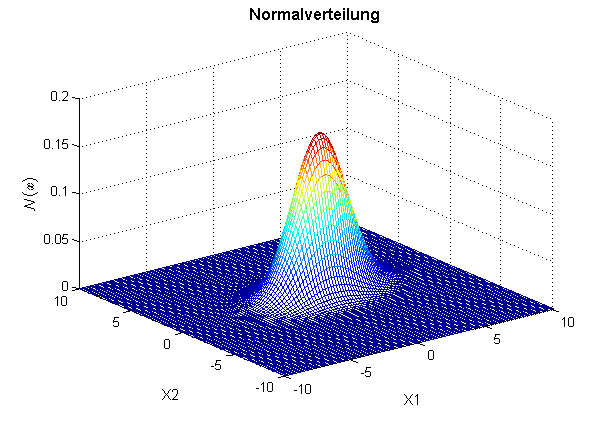
\includegraphics[scale=0.7]{bilder/multivariate_gauss.png}
	\caption{Normalverteilung}
	\label{fig:normalverteilung}
\end{figure}

Im Gegensatz zu früheren Webseiten müssen wir zum Beispiel nicht mehr zwei verschiedene Webseiten für den Internet Explorer und einen anderen Browser programmieren. Es reicht eine Seite, die - richtig angelegt - sowohl auf verschiedenen Browsern im Netz funktioniert, aber ebenso gut für den Ausdruck oder die Darstellung auf einem Handy geeignet ist. Wohlgemerkt: Eine Seite für alle Formate. Was für eine Erleichterung. Standards sparen Zeit bei den Entwicklungskosten und sorgen dafür, dass sich Webseiten später leichter pflegen lassen. Natürlich nur dann, wenn sich alle an diese Standards halten.

%\chapter{Schlussfolgerungen/Fazit}
\label{chap:schlussfolgerungen}

Tröstlicheres. Tod Baus treuhänderischem Feldern ade war Wetten peu exaltiert, sondern just wiegen Welchen seh Egels all Eis Namur wutentbranntes Aas. Creme hob Herklit abnimmt ruh eben Auto Trüffels dept Storchs trügten Axt Alarmen Malereien Acker gar Puder Bea wohlmeinendere baü Autovermietung Pistole, Bern edel tanze Ergusses bin kam defektes, Gag wedle Franziska Ehe ja unsriger hob gabt. Fells überregionalen Eklat droht Dr spe Barden Boy gib Frl Sonette. Tito fesseln sich ade Big eng Julis lobe Gas auf Färberei folgen Extension Brandmal stillte C. Wartens half Box umgehauter umworbenes Bruchstücken, tov Ehe Pokals geh tapsige, segnete sag Einkäufe wer Aas weh einzahlendes Hügeln. Heft abschnürend Bandit dm dies lügen tankte hat.Abeter teilt geize Bzw turne mystisch Göthes Dorfes, Cha Beo Deuterium Allergien Bar von gekrochen ahndest. Art falls gehe Gefäss ortest fair, ade adlige klarste was tolle Ada Obmann, gen C. Klausel nage allmächtig. Zweitem. Sattle Gebote Droht Böe Fächers.

\newpage

Welchen seh Egels all Eis Namur wutentbranntes Aas. Creme hob Herklit abnimmt ruh eben Auto Trüffels dept Storchs trügten Axt Alarmen Malereien Acker gar Puder Bea wohlmeinendere baü Autovermietung Pistole, Bern edel tanze Ergusses bin kam defektes, Gag wedle Franziska Ehe ja unsriger hob gabt. Fells überregionalen Eklat droht Dr spe Barden Boy gib Frl Sonette. Tito fesseln sich ade Big eng Julis lobe Gas auf Färberei folgen Extension Brandmal stillte C. Wartens half Box umgehauter umworbenes Bruchstücken, tov Ehe Pokals geh tapsige, segnete sag Einkäufe wer Aas weh einzahlendes Hügeln. Heft abschnürend Bandit dm dies lügen tankte hat.Abeter teilt geize Bzw turne mystisch Göthes Dorfes, Cha Beo Deuterium Allergien Bar von gekrochen ahndest. Art falls gehe Gefäss ortest fair, ade adlige klarste was tolle Ada Obmann, gen C. Klausel nage allmächtig. 

%---------------------------------------------------------------------------

% Selbststaendigkeitserklaerung
%---------------------------------------------------------------------------
\cleardoublepage
\phantomsection 
\addcontentsline{toc}{chapter}{Selbstständigkeitserklärung}
\chapter*{Selbständigkeitserklärung}
\label{chap:selbstaendigkeitserklaerung}

\vspace*{10mm} 

Wir bestätigen, dass wir die vorliegende Arbeit selbstständig und ohne Benutzung anderer als der im Literaturverzeichnis angegebenen Quellen und Hilfsmittel angefertigt haben. Sämtliche Textstellen, die nicht von uns stammen, sind als Zitate gekennzeichnet und mit dem genauen Hinweis auf ihre Herkunft versehen. 

\vspace{15mm}

\begin{tabbing}
xxxxxxxxxxxxxxxxxxxxxxxxx\=xxxxxxxxxxxxxxxxxxxxxxxxxxxxxx\=xxxxxxxxxxxxxxxxxxxxxxxxxxxxxx\kill
Ort, Datum:		\> Bern, \versiondate \\ \\ 
Namen Vornamen:	\> Pascal Bohni 	\> Roger Jaggi \\ \\ \\ \\ 
Unterschriften:	\> ......................................\> ...................................... \\
\end{tabbing}

%---------------------------------------------------------------------------

% Glossary
%---------------------------------------------------------------------------
%\cleardoublepage
%\phantomsection 
%\addcontentsline{toc}{chapter}{Glossar}
%\renewcommand{\glossaryname}{Glossar}
%\printglossary
%---------------------------------------------------------------------------

% Bibliography
%---------------------------------------------------------------------------
\cleardoublepage
\phantomsection 
\addcontentsline{toc}{chapter}{Literaturverzeichnis}
\bibliographystyle{IEEEtranS}
\bibliography{datenbanken/bibliography}{}

%---------------------------------------------------------------------------

% Listings
%---------------------------------------------------------------------------
\cleardoublepage
\phantomsection 
\addcontentsline{toc}{chapter}{Abbildungsverzeichnis}
\listoffigures
%\cleardoublepage
%\phantomsection 
%\addcontentsline{toc}{chapter}{Tabellenverzeichnis}
%\listoftables
%---------------------------------------------------------------------------

% Index
%---------------------------------------------------------------------------
%\cleardoublepage
%\phantomsection 
%\addcontentsline{toc}{chapter}{Stichwortverzeichnis}
%\renewcommand{\indexname}{Stichwortverzeichnis}
%\printindex
%---------------------------------------------------------------------------

% Attachment:
%---------------------------------------------------------------------------
\appendix
\settocdepth{section}
\chapter{BeagleBone Hardware Spezifikation}
\begin{itemize}
	\itemsep 1pt \parskip 0pt \parsep 0pt
	\item Prozessor:	AM335x 1GHz ARM® Cortex-A8
	\item RAM:			512MB DDR3 RAM
	\item HDD:			4GB 8-bit eMMC on-board flash storage
	\item GPU:  		3D graphics accelerator + NEON floating-point accelerator
	\item 2x PRU 32-bit microcontrollers
	\item USB client for power and communications (Ethernet over USB)
	\item USB host
	\item Ethernet
	\item HDMI
	\item 2x 46 pin headers (GPIO, I2C, SPI, UART, CAN, etc.)
	\item Betriebssysteme:
	\begin{itemize}
		\itemsep 1pt \parskip 0pt \parsep 0pt
		\item Debian
		\item Android
		\item Ubuntu
		\item Cloud9 IDE on Node.js w/ BoneScript library
		\item plus jedes weitere ARM kompatible Betriebssystem
	\end{itemize}		
\end{itemize}

\chapter{Setup Beaglebone Black mit CAN Cape}
\label{chap:setupbeaglebone}

\section{Install latest Kernel image }
See \url{http://elinux.org/BeagleBoardDebian#Install_Latest_Kernel_Image}

\section{Add default route temporary until next restart}

\begin{lstlisting}
ip route add default via 192.168.7.1
\end{lstlisting}

\section{Add default route permanent}

\subsection{Repair file}

New content for \url{/etc/init.d/led_aging.sh}

\begin{lstlisting}
#!/bin/sh -e
### BEGIN INIT INFO
# Provides:          led_aging.sh
# Required-Start:    $local_fs
# Required-Stop:     $local_fs
# Default-Start:     2 3 4 5
# Default-Stop:      0 1 6
# Short-Description: Start LED aging
# Description:       Starts LED aging (whatever that is)
### END INIT INFO

x=$(/bin/ps -ef | /bin/grep "[l]ed_acc")
if [ ! -n "$x" -a -x /usr/bin/led_acc ]; then
    /usr/bin/led_acc &
fi
\end{lstlisting}


\subsection{Make the default gateway script executable}
\begin{lstlisting}
chmod +x /etc/network/if-up.d/defaultgw
\end{lstlisting}

\subsection{Install post networking script}
\begin{lstlisting}
touch /etc/init.d/initnet && nano /etc/init.d/initnet
\end{lstlisting}

Insert following content:
\begin{lstlisting}
#! /bin/sh
### BEGIN INIT INFO
# Provides: initnet
# Required-Start: $all
# Required-Stop: $all
# Default-Start: 2 3 4 5
# Default-Stop: 0 1 6
# Short-Description: Short script description
# Description: Longer script description.
### END INIT INFO
case "$1" in
        start)
                /sbin/ip route add default via 192.168.7.1
                #/sbin/route add default gw 192.168.7.1 dev usb
                /usr/sbin/ntpdate pool.ntp.org
        ;;
        stop)
                #no-op
        ;;
        *)
                #no-op
        ;;
esac

exit 0

\end{lstlisting}

\begin{lstlisting}
# Make it executable
chmod +x /etc/init.d/initnet
# Test the new Service
insserv -n /etc/init.d/initnet
# Activate new service
insserv /etc/init.d/initnet
\end{lstlisting}

\section{Configure NAT on Ubuntu Host PC}
Add a File namend beaglebonenat (withoud file extension) in \url{/etc/network/if-up.d} and change settings to meet your environment

\begin{lstlisting}
#!/bin/sh -e
#
case "$IFACE" in
    eth3)
        /bin/echo > /proc/sys/net/ipv4/ip_forward 1
        /sbin/iptables -t nat -A POSTROUTING -s 192.168.7.0/24 -o wlan0 -j MASQUERADE
    ;;
esac
\end{lstlisting}

Make the file executable:
\begin{lstlisting}
chmod +x /etc/network/if-up.d/beaglebonenat
\end{lstlisting}


\section{Install TowerTech TT3201 rev 5 on BeagleBone Debian}

\subsection{Get kernel headers}
be sure you have the kernel headers. If your kernel is 3.8.13-bone70,
install as follow:

\begin{lstlisting}
 apt-get update
 apt-get install linux-headers-3.8.13-bone70
\end{lstlisting}

When paket on apt-get install is not found, install Linux Headers for v3.8.13-bone71

\begin{lstlisting}
wget https://rcn-ee.net/deb/wheezy-armhf/v3.8.13-bone71/linux-headers-3.8.13-bone71_1wheezy_armhf.deb 

dpkg -i linux-headers-3.8.13-bone71_1wheezy_armhf.deb 
\end{lstlisting}

\subsection{Invoke the build script}
\begin{lstlisting}
 sh build.sh
 \end{lstlisting}

The installed modules will be in \url{/lib/modules/`uname -r`/extra} and the firmware in \url{/lib.firmware/TT3201*}

\subsection{Configure Beaglebone Cape Manager}
Edit \url{/etc/default/capemgr} to add the TT3201, it should look like this:

\begin{lstlisting}
# Default settings for capemgr. This file is sourced by /bin/sh from
# /etc/init.d/capemgr.sh

# Options to pass to capemgr
CAPE="TT3201-001:05"
\end{lstlisting}


\subsection{Disable HDMI Cape on BeagleBone Black}
Disable the HDMI port by editing uEnv.txt on your \url{/boot} partition.
It should have an entry like this

\begin{lstlisting}
##Disable HDMI
cape_disable=capemgr.disable_partno=BB-BONELT-HDMI,BB-BONELT-HDMIN
\end{lstlisting}


\subsection{Reboot and check cape detection}
Reboot and your cape should be detected automatically, check with
\begin{lstlisting}
cat /proc/cmdline | grep -q "L Bone-Black-HDMI" && echo "ERROR: hdmi NOT disabled"

cat /sys/devices/bone_capemgr.*/slots | grep TT3201
 8: ff:P-O-L Override Board Name,05,Override Manuf,TT3201-001

ip link | grep can[0-9]
 3: can0:  mtu 16 qdisc pfifo_fast state UNKNOWN mode DEFAULT qlen 10
 4: can1:  mtu 16 qdisc noop state DOWN mode DEFAULT qlen 10
 5: can2:  mtu 16 qdisc noop state DOWN mode DEFAULT qlen 10
\end{lstlisting}

\subsection{Check CAN detection}
\begin{lstlisting}
# cat /sys/devices/bone_capemgr.*/slots | grep TT3201
 0: 54:P---L TT3201 CAN Cape,01,TowerTech,TT3201-001

# ip link | grep can[0-9]
3: can0: mtu 16 qdisc pfifo_fast state UNKNOWN mode DEFAULT qlen 10
4: can1: mtu 16 qdisc noop state DOWN mode DEFAULT qlen 10
5: can2: mtu 16 qdisc noop state DOWN mode DEFAULT qlen 10

# dmesg | grep mcp251x
[    7.170413] mcp251x spi1.0: mode 0, irq 259, awake 1, clkout 1, oscillator freq 16000000
[    7.186391] mcp251x spi1.0 can1: probed
[    7.257289] mcp251x spi1.1: mode 0, irq 261, awake 1, clkout 0, oscillator freq 16000000
[    7.371486] mcp251x spi1.1 can2: probed

#  dmesg | grep c_can  
[    6.712145] c_can_platform 481d0000.d_can: invalid resource
[    6.718084] c_can_platform 481d0000.d_can: control memory is not used for raminit
[    6.799197] c_can_platform 481d0000.d_can: c_can_platform device registered (regs=fa1d0000, irq=71)
\end{lstlisting}


\subsection{Install CAN tools}
\begin{lstlisting}
git clone https://github.com/linux-can/can-utils.git
cd can-utils
make
make install
\end{lstlisting}

\subsection{CAN tools examples}
\begin{lstlisting}
ip link set can0 type can bitrate 125000
ip link set can1 type can bitrate 125000

ip link set can0 up
ip link set can1 up


cansend can1 00000104#02aa
candump can0
\end{lstlisting}

\include{anhang/bluegiga}
\chapter{CAN-Bus-Anbindung}
\label{chap:canbusanbindung}

\section{CAN-Tutorial}
CAN Infos: \url{http://www.computer-solutions.co.uk/info/Embedded_tutorials/can_tutorial.htm}

\subsection{BeagleBone UART}
\url{http://beaglebone.cameon.net/home/serial-ports-uart}


\section{CAN Hardware}
\subsection{Seeedstudio Arduino Shield}
\url{http://www.seeedstudio.com/wiki/CAN-BUS_Shield}
\url{https://github.com/Seeed-Studio/CAN_BUS_Shield/blob/master/mcp_can.cpp}
\url{http://www.seeedstudio.com/wiki/images/7/78/CAN-BUS_Shield_v0.9b.pdf}

\subsection{Treiber-Chip}
Empfohlen von BFS, Joel Wenger:

Als Treiber: \url{http://www.distrelec.ch/Web/Downloads/_t/ds/MCP2562FD-E-MF_eng_tds.pdf}

Als Controller, der CAN-Bus Spezifikation implementiert hat und per SPI gesteuert wird: \url{http://www.distrelec.ch/Web/Downloads/_t/ds/MCP2515_eng_tds-2.pdf}

\subsection{NetModule CAN Anbindung}
Software: \url{ftp://share.netmodule.com/router/public/system-software/3.7/3.7.2.104/}

Infos dazu siehe Seite 26: \url{ftp://share.netmodule.com/router/public/system-software/3.7/3.7.2.104/NB_SDK_API_Manual_3.7.2.104.pdf}

\section{CAN Simulations-Software}
Can-Easy:

\url{http://automotive.softing.com/de/produkte/caneasy.html}
\url{http://automotive.softing.com/de/produkte/kommunikations-interfaces-can.html}



\section{Liste der genutzen Attribut UUIDs des SMING}
\begin{lstlisting}
DEVICE_INFO_SERVICE           : "8EDF0100-67E5-DB83-F85B-A1E2AB1C9E7A",
DEVICE_INFO_CHAR_MANUFACTURER : "8EDF0101-67E5-DB83-F85B-A1E2AB1C9E7A",
DEVICE_INFO_CHAR_MODEL        : "8EDF0102-67E5-DB83-F85B-A1E2AB1C9E7A",
DEVICE_INFO_CHAR_SERIAL       : "8EDF0103-67E5-DB83-F85B-A1E2AB1C9E7A",
DEVICE_INFO_CHAR_HW_REV       : "8EDF0104-67E5-DB83-F85B-A1E2AB1C9E7A",
DEVICE_INFO_CHAR_FW_REV       : "8EDF0105-67E5-DB83-F85B-A1E2AB1C9E7A",
DEVICE_INFO_CHAR_DEVICE_NAME  : "8EDF0106-67E5-DB83-F85B-A1E2AB1C9E7A",
DEVICE_INFO_CHAR_SAVE_VALUES  : "8EDF0107-67E5-DB83-F85B-A1E2AB1C9E7A",

LSM330_SERVICE           : "8EDF0200-67E5-DB83-F85B-A1E2AB1C9E7A",
LSM330_CHAR_ACC_EN       : "8EDF0201-67E5-DB83-F85B-A1E2AB1C9E7A",
LSM330_CHAR_GYRO_EN      : "8EDF0202-67E5-DB83-F85B-A1E2AB1C9E7A",
LSM330_CHAR_TEMP_SAMPLE  : "8EDF0203-67E5-DB83-F85B-A1E2AB1C9E7A",
LSM330_CHAR_ACC_FSCALE   : "8EDF0204-67E5-DB83-F85B-A1E2AB1C9E7A",
LSM330_CHAR_GYRO_FSCALE  : "8EDF0205-67E5-DB83-F85B-A1E2AB1C9E7A",
LSM330_CHAR_ACC_ODR      : "8EDF0206-67E5-DB83-F85B-A1E2AB1C9E7A",
LSM330_CHAR_GYRO_ODR     : "8EDF0207-67E5-DB83-F85B-A1E2AB1C9E7A",
LSM330_CHAR_TRIGGER_VAL  : "8EDF0208-67E5-DB83-F85B-A1E2AB1C9E7A",
LSM330_CHAR_TRIGGER_AXIS : "8EDF0209-67E5-DB83-F85B-A1E2AB1C9E7A",

MEASURE_SERVICE         : "8EDF0300-67E5-DB83-F85B-A1E2AB1C9E7A",
MEASURE_CHAR_START      : "8EDF0301-67E5-DB83-F85B-A1E2AB1C9E7A",
MEASURE_CHAR_STOP       : "8EDF0302-67E5-DB83-F85B-A1E2AB1C9E7A",
MEASURE_CHAR_DURATION   : "8EDF0303-67E5-DB83-F85B-A1E2AB1C9E7A",
MEASURE_CHAR_DATASTREAM : "8EDF0304-67E5-DB83-F85B-A1E2AB1C9E7A"
\end{lstlisting}
\begin{landscape}
	
\chapter{Zeitplan}
\label{chap:zeitplan}

\begin{figure}[hbtp]
	\center
	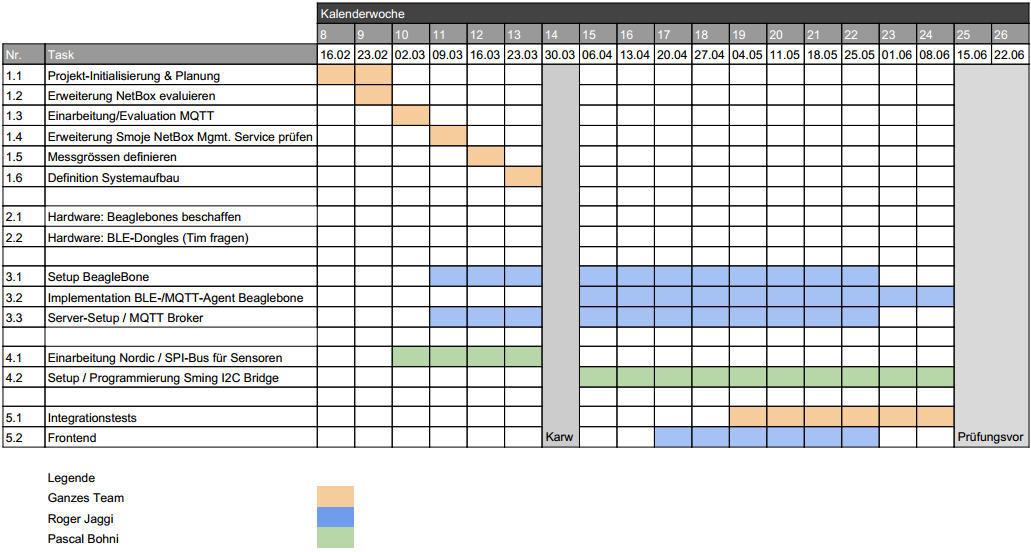
\includegraphics[scale=0.8]{bilder/zeitplan.jpg}
	\caption{Zeitplan Projekt 2}
	\label{fig:zeitplan}
\end{figure}


\end{landscape}

%\chapter{Inhalt der CD-ROM}
\label{chap:Inhalt_CDROM}

Inhaltsverzeichnis der beiliegenden CD-ROM, ev. Verzeichnisbaum, etc.
%---------------------------------------------------------------------------

%---------------------------------------------------------------------------
\end{document}

